\documentclass{ctexart}

\usepackage{amsmath,mathtools}
\usepackage[all,pdf]{xy}
\usepackage{pstricks-add}
\usepackage{tikz}
\usepackage{siunitx}
\usepackage{asymptote}

\begin{document}
\xymatrix{
  a & b & a+b \\
  1 & 2 & 3 \\
}

\xymatrix{
  a & b\ar[rd] & a+b \\ % 指向右下方
  1 & 2 & 3\ar"1,1"     % 指向 (1,1)
  \ar"1,1";"2,2"  % 直接从 (1,1) 到 (2,2)
}

\xymatrix{
  A\ar[r]^{\alpha} & B\ar[d]_{\beta} \\
  C\ar[ur]|{\Sigma} & D \\
}

\xymatrix{
  A\ar[rd]|\hole & B \\
  C\ar[ru] & D
}

\xymatrix{
  A \ar[r]^>{f} & B \\
  C \ar[r]^>>{g} & D \\
  E \ar[r]^(0.6){h} & F
}

\xymatrix{
  A \ar[drr]|!{[d];[r]}\hole & B & \\
  C \ar[ur] & & D
}

\begin{equation}
\begin{gathered}
\xymatrix{
S\ar[r]^{f_s} \ar[d]_{\lambda} & T\ar[d]_{\bar{\lambda}} \\
S'\ar[r]_{f_{s'}} & T' \\
}
\end{gathered}
\end{equation}

\begin{equation}
\begin{gathered}
\xymatrix{
S\ar[r]^{f_s} \ar[d]_{\lambda} & T\ar[d]^{\bar{\lambda}} \\
S'\ar[r]_{f_{s'}} & T' \\
}
\end{gathered}
\end{equation}

映射 $\xymatrix@1{A\ar[r]^{f} & B}$ 是同态.

映射 $\xymatrix{A\ar[r]^{f} & B}$ 是同态.

\[ \xymatrix{
 A \ar@/^/[r]^{\phi} & B \ar@/^/[l]^{\psi}
 } \]

\[ \xymatrix{
  A \ar@<.5ex>[r]^f &
  \ar@<.5ex>[l]^g B
} \]

\[ \xymatrix@=2cm{
  *[F]{A} \ar[r]^*+[F=]{k} & *+[o][F]{B}
} \]

    \xymatrix{
      *++=[o][F]\txt{猫猫} \ar@{<->}[r] &
      *+[F]\txt{狗\\狗}
    }

    \xymatrix{
      *+[F.]{\composite{*+[o][F]{a\quad} * *+[F]{\quad b}}} \ar[r]
        & *+[F]{c}
    }

    \xymatrix@R=2ex{
      A \ar[drr]& B & C \\
      D & E & F
    }

    \xymatrix@ru{
      A \ar[r] & B \ar[d] \\
      C \ar[u] & D \ar[l]
    }

\xymatrix{
 A'\ar[rd]\ar[rr] & &  B'\ar[rd]\ar[dd]|\hole & \\
    & A\ar[rr] & & B\ar[dd] \\
 C'\ar[uu]\ar[rd] &   &  D'\ar[ll]|\hole \ar[rd]  &   \\
    & C\ar[uu] &       & D\ar[ll]
}
\newpage

直线
\psline(0,0)(1,1em)(1.5,0)
直线

    直线
    \begin{pspicture}(1.5,1em)
    \psline(0,0)(1,1em)(1.5,0)
    \end{pspicture}
    直线

    \begin{pspicture}(-1.2,-1.2)(1.2,1.2)
      \psaxes(0,0)(-1.2,-1.2)(1.2,1.2)
      \pscircle(0,0){1}
    \end{pspicture}

    \psset{linewidth=0.4pt}
    \begin{pspicture}(-1.2,-1.2)(1.2,1.2)
      \psaxes[labels=none,ticks=none]
        {->}(0,0)(-1.2,-1.2)(1.2,1.2)
      \pscircle[linewidth=0.8pt](0,0){1}
    \end{pspicture}

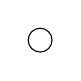
\begin{tikzpicture}
\draw (0,0) circle (1ex);
\end{tikzpicture}

圆形
\tikz \draw (0,0) circle (1ex);

\tikz \fill (0,0) circle (1ex);

\tikz \filldraw[thick,fill=gray]
  (0,0) circle (0.5cm);

Hello world!
    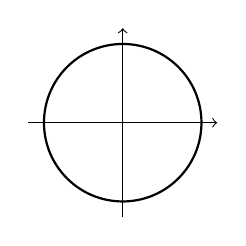
\begin{tikzpicture}
      \draw[->] (-1.2,0) -- (1.2,0);
      \draw[->] (0,-1.2) -- (0,1.2);
      \draw[thick] (0,0) circle (1);
    \end{tikzpicture}
  
    \tikz\draw (30:0.5) arc (30:150:0.5);

    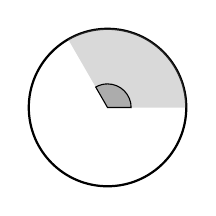
\begin{tikzpicture}
      \draw[thick] (0,0) circle (1);
      \fill[fill=gray, fill opacity=0.3]
        (0,0) -- (0:1) arc (0:120:1) -- cycle;
      \filldraw[fill=gray,fill opacity=0.5]
        (0,0) -- (0:0.3) arc (0:120:0.3) -- cycle;
    \end{tikzpicture}
  
    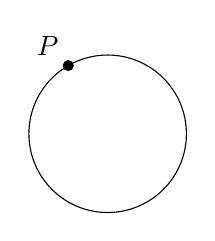
\begin{tikzpicture}
    \draw (0,0) circle (1);
    \fill (120:1) circle (2pt);
    \node[above left] (P) at (120:1) {$P$};
    \end{tikzpicture}

    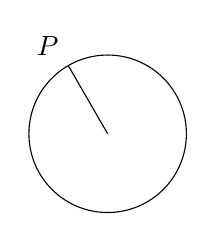
\begin{tikzpicture}
    \draw (0,0) circle (1);
    \coordinate[label=120:$P$] (P) at (120:1);
    \draw (0,0) -- (P);
    \end{tikzpicture}

    % \usepackage{siunitx}
    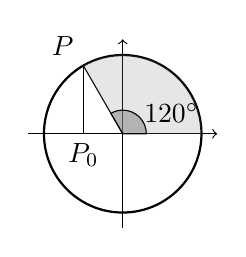
\begin{tikzpicture}
      \newcommand\iangle{120}
      \draw[->] (-1.2,0) -- (1.2,0);
      \draw[->] (0,-1.2) -- (0,1.2);
      \draw[thick] (0,0) circle (1);
      \coordinate[label=\iangle:$P$] (P) at (\iangle:1);
      \coordinate[label=below:$P_0$] (P0) at (P |- 0,0);
      \draw (0,0) -- (P);
      \draw (P) -- (P0);
      \fill[fill=gray,fill opacity=0.2]
        (0,0) -- (0:1) arc (0:\iangle:1) -- cycle;
      \filldraw[fill=gray,fill opacity=0.5]
        (0,0) -- (0:0.3) arc (0:\iangle:0.3) -- cycle;
      \node[right] at (\iangle/2:0.3) {\ang{\iangle}};
    \end{tikzpicture}

    \begin{tikzpicture}
      % 从 0 度到 360 度的正弦函数曲线,rad 函数和单位 r 把度转换为弧度
      \draw[domain=0:rad(360)] plot (\x, {sin(\x r)});
    \end{tikzpicture}

    \begin{tikzpicture}
    \draw (0,0) -- (2,0) node[right] {右};
    \draw (0,-1) -- node[above] {连线} (2,-1);
    \end{tikzpicture}

    \begin{tikzpicture}
    % 坐标轴
    \draw[->] (0,0) -- ({rad(210)}, 0);
    \draw[->] (0,-1.2) -- (0,1.2);
    % 文字标签与刻度
    \foreach \t in {0, 90, 180} {                           % 遍历三个角度
      \draw ({rad(\t)}, -0.05) -- ({rad(\t)}, 0.05);        % 画刻度线
      \node[below, outer sep=2pt, fill=white, font=\small]  % 标注横轴角度
        at ({rad(\t)}, 0) {\ang{\t}};
    }
    \foreach \y in {-1,1} {\draw (-0.05,\y) -- (0.05,\y);}  % 纵轴刻度
    \end{tikzpicture}

    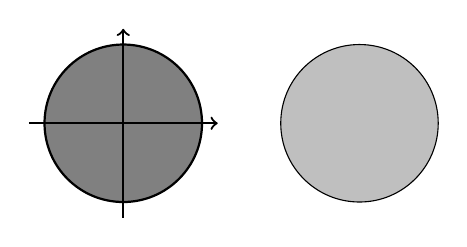
\begin{tikzpicture}[fill=lightgray] % 全局选项
    \begin{scope}[thick,->,fill=gray,xshift=-3cm] % 区块内整体向左平移
      \filldraw (0,0) circle (1);
      \draw (-1.2,0) -- (1.2,0);
      \draw (0,-1.2) -- (0,1.2);
    \end{scope}
    \filldraw (0,0) circle (1); % 原位置
    \end{tikzpicture}

    \begin{figure}
    \centering
    % \usepackage{siunitx}
    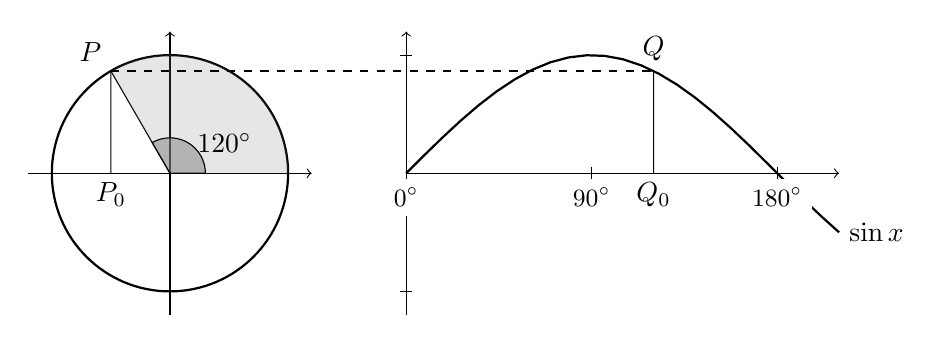
\begin{tikzpicture}[scale=1.5] % 整体放大坐标,但不影响字号
      \newcommand\iangle{120}
      % 左边的单位圆
      \begin{scope}[xshift=-2cm]
        \draw[->] (-1.2,0) -- (1.2,0);
        \draw[->] (0,-1.2) -- (0,1.2);
        \draw[thick] (0,0) circle (1);
        \coordinate[label=\iangle:$P$] (P) at (\iangle:1);
        \coordinate[label=below:$P_0$] (P0) at (P |- 0,0);
        \draw (0,0) -- (P);
        \draw (P) -- (P0);
        \fill[fill=gray,fill opacity=0.2]
          (0,0) -- (0:1) arc (0:\iangle:1) -- cycle;
        \filldraw[fill=gray,fill opacity=0.5]
          (0,0) -- (0:0.3) arc (0:\iangle:0.3) -- cycle;
        \node[right] at (\iangle/2:0.3) {\ang{\iangle}};
      \end{scope}
      % 右边的函数图
      \draw[->] (0,0) -- ({rad(210)}, 0);
      \draw[->] (0,-1.2) -- (0,1.2);
      \draw[thick, domain=0:rad(210)] plot (\x, {sin(\x r)})
        node[right] {$\sin x$};
      \foreach \t in {0, 90, 180} {
        \draw ({rad(\t)}, -0.05) -- ({rad(\t)}, 0.05);
        \node[below, outer sep=2pt, fill=white, font=\small]
          at ({rad(\t)}, 0) {\ang{\t}};
      }
      \foreach \y in {-1,1} {\draw (-0.05,\y) -- (0.05,\y);}
      \coordinate[label=above:$Q$] (Q) at ({rad(\iangle)}, {sin(\iangle)});
      \coordinate[label=below:$Q_0$] (Q0) at (Q |- 0,0);
      \draw (Q) -- (Q0);
      \draw[dashed] (P) -- (Q);
    \end{tikzpicture}
    \caption{正弦函数与单位圆(\textsf{TikZ} 实现)}
    \label{fig:tikzsine}
    \end{figure}


    % \usepackage{asymptote}
    \begin{asy}
    real r = 0.8cm;
    for (int i = 0; i < 360; i+=10)
        draw(circle(dir(i)*r, r));
    \end{asy}
\end{document} 